% === Notes from Elvis ===

%%%%%%%%%%%%%%%%%%%%%%%%%%%%%%%%%%%%%%%%%%%%%%%%%%%%%%%%%%%%%%%%%%%%%%%%%%%%%%%%
% The above line is 80 characters long. Try to keep it under this width.

% There are 3 ways of highlighting:
%  o \texttt
%      o Folders
%      o Files
%      o Program names
%  o \emph
%      o Company names
%      o New concepts that are introduced
%  o \textcode (\texttt with grey background)
%      o Commands
%      o Command output

%\chapter
%    \section
%        \subsection
%            \subsubsection
%            \paragraph

% === Setup ===

% Needed and Layout
\documentclass[a4paper,11pt]{report}
\usepackage[utf8]{inputenc} % utf8 encoding
\usepackage{amsfonts}
\usepackage[T1]{fontenc} % use for allowing < and > in cleartext
\usepackage[margin=2.5cm]{geometry}

% Lists
\usepackage{verbatim}   % useful for program listings
\usepackage{enumitem}
\usepackage[ampersand]{easylist}

% Creating more compact lists
\let\olditemize\itemize
\renewcommand{\itemize}{
    \olditemize
    \setlength{\itemsep}{1pt}
    \setlength{\parskip}{0pt}
    \setlength{\parsep}{0pt}
}


% Creating my own inline code font
\newcommand{\textcode}[1]{
    \fboxsep=1pt
    \texttt{\colorbox{gray!20}{#1}}
}

% Recreating the figure thingy
\newcommand{\figa}{
    \begin{figure}[!htpb]
    \centering
}
\newcommand{\figb}[2]{
    \caption{#1}
    \label{#2}
    \end{figure}
}


% Math
\usepackage{mathtools}   % need for subequations
\usepackage{xfrac}       % Fractions  like 1/4 via \sfrac

% Graphics
\usepackage{graphicx}   % need for figures
\usepackage{color}      % use if color is used in text 
\usepackage{xcolor}     % use for text background color
\usepackage{tikz}
\usetikzlibrary{arrows}
\usepackage{float}

% Other
\usepackage{todonotes}
\usepackage{pdfpages}
\usepackage{subcaption}
\usepackage{latexsym}
\usepackage{fixltx2e}    % use for textsubscript
\usepackage[titletoc,title]{appendix}
\usepackage[framemethod=tikz]{mdframed}
\usepackage[titletoc,title]{appendix}
\usepackage{epstopdf}

% Code listing
\usepackage{listings} % For inserting code from file (I think)
\usepackage{algorithm}
\usepackage{algpseudocode}
\renewcommand{\algorithmicforall}{\textbf{for each}}
\makeatletter
\def\BState{\State\hskip-\ALG@thistlm}
\makeatother

\DeclareCaptionFormat{algor}{%
  \hrulefill\par\offinterlineskip\vskip1pt%
    \textbf{#1#2}#3\offinterlineskip\hrulefill}
\DeclareCaptionStyle{algori}{singlelinecheck=off,format=algor,labelsep=space}
\captionsetup[algorithm]{style=algori}

% URLs ? maybe
%\usepackage{hyperref}
\usepackage{url}
\usepackage[hypcap=false]{caption}


% for the \lstinputlisting for code blocks
\definecolor{codegreen}{rgb}{0,0.6,0}
\definecolor{codegray}{rgb}{0.5,0.5,0.5}
\definecolor{codepurple}{rgb}{0.58,0,0.82}
\definecolor{backcolour}{rgb}{1.0,1.0,1.0}
\lstdefinestyle{mystyle}{
  backgroundcolor=\color{backcolour},   
  commentstyle=\color{codegreen},
  keywordstyle=\color{magenta},
  numberstyle=\tiny\color{codegray},
  stringstyle=\color{codepurple},
  basicstyle=\ttfamily\footnotesize,
  breakatwhitespace=false,         
  breaklines=true,                 
  captionpos=b,                    
  keepspaces=true,                 
  numbers=left,                    
  numbersep=1pt,                  
  showspaces=false,                
  showstringspaces=false,
  showtabs=false,                  
  tabsize=2
}
\lstset{style=mystyle}

\begin{document}

% Configuration
\setlength{\parindent}{0cm}
\setlength{\unitlength}{1mm}

% Front Page
\date{September 1st 2015\\ IT University of Copenhagen}
\title{A Quantitative Analysis of Variability Bugs in Linux}
\author{Elvis Flesborg\\
\texttt{efle@itu.dk}}
\clearpage\maketitle
\thispagestyle{empty}
\newpage

%%%%%%%%%%%%%%%%%%%%%%%%%%%%%%%%%%%%%%%%%%%%%%%%%%%%%%%%%%%%%%%%%%%%%%%%%%%%%%%%
%                           TABLE OF CONTENTS
%%%%%%%%%%%%%%%%%%%%%%%%%%%%%%%%%%%%%%%%%%%%%%%%%%%%%%%%%%%%%%%%%%%%%%%%%%%%%%%%
\tableofcontents
\thispagestyle{empty}



\newpage

\setcounter{page}{1}


\begin{abstract}
    \emph{---Leave blank until the end---}

\end{abstract}


\chapter{Introduction}
\emph{---Leave blank until the end---}


% TODO
\begin{itemize}
    \item \underline{\textbf{TODO}}
        \item Explain about representative samples
\end{itemize}


%%%%%%%%%%%%%%%%%%%%%%%%%%%%%%%%%%%%%%%%%%%%%%%%%%%%%%%%%%%%%%%%%%%%%%%%%%%%%%%%
%                           BACKGROUND
%%%%%%%%%%%%%%%%%%%%%%%%%%%%%%%%%%%%%%%%%%%%%%%%%%%%%%%%%%%%%%%%%%%%%%%%%%%%%%%%
\newpage
        \chapter{Background}

A \emph{Linux} operating system is often referring to a a \emph{GNU/Linux} 
operating system, where the Linux part of \emph{GNU/Linux} is the Linux kernel, 
and the \emph{GNU} part is a software bundle with utilities (eg. a shell, a 
compiler, etc...) \cite{gnu_pack}. Both is 
needed, to have a working operating system. 
\\

This report will only focus on the \emph{Linux kernel}, and not the \emph{GNU} 
bundle.


        \section{The Linux Kernel and Variability}

Many software products are configurable in some way. This creates the 
possibility of tailoring the software to suit different needs. For example 
different kinds of hardware, or different functionalities. 

In Linux this is done before compilation, at a preprocessing step. The Linux 
kernel in its entirety is not a valid program, it will have to be preprocessed 
to make sense of the source code.
This is done by the preprocessing tool (in this case \emph{gcc}).
    \cite[p. 1]{IntDatSPL}
    \footnote{\url{http://gcc.gnu.org/}}
    \footnote{cite some ifdef thing (look at IntDatSPL pg. 1 [3][4]}
\\

This is also called \emph{variability} in software and a software product of 
this type is called \emph{Software Product Lines} (SPL). When different 
software programs can be derived from the same source code base. 

Software with a high-degree of variability is usually refered to as 
\emph{Variability-Intensive Systems} or \emph{VISs}. Other examples of 
\emph{VISs} are \emph{Eclipse}, \emph{Amazon Elastic Compute Service}, and 
\emph{Drupal Content Management Framework} 
    \cite[p. 1]{VarTesDrupal}
to name a few.
\\

The Linux kernel is very configurable. In the configuration files (the Kconfig 
files), there is a total of 14,387 different features, that can be configured.
    \footnote {14,387 across all architectures, with an average of 9,984 per 
        architecture}
It is the open source software product with the highest degree of variability.

This high degree of variability has also had an impact on the use cases for the 
Linux kernel. Linux is used for anything from small embedded devices (like car 
GPSs, and cell phones) to supercomputers.
In fact 98\% of the top 500 supercomputers in the world run a Linux distibution
    \cite{top500}
.
\\

This high variability rate makes maintaining the code somewhat harder to 
grasp, and this makes the code base more error prone. So what you get in 
scalability you pay for in complexity of maintaining the code. 
    \footnote{Refer to Jean's project maybe}
    \footnote{Also refer to a paper that andrzej made about industrial 
        something. It said something about how much more efficient the code was,
        when variability was there.}


        \section{Linux Kernel Development}

\begin{center}
    \emph{
        Comment from the Linux team or something...
    }
\end{center}


        \subsection*{Stable and Mainline tree}

The Linux kernel development cycle has approximately 2$\sfrac{3}{4}$ months 
from one stable release to the next stable release
    \cite{crystalball}
.
In the meantime, \emph{Release Candidates (RCs)}, are released approximately 
once every week.

Then, when the top maintainers of the mainline tree think that the kernel is 
stable enough, a new stable version is created, and the whole process is 
repeated.


        \subsection*{linux-next tree}

Then there is the \emph{linux-next} tree. It is a \emph{git} repository, which 
merges over 200 other \emph{git} repositories
    \cite{nextTrees}
, which 
are all based on the \emph{mainline} tree. The \emph{linux-next} tree is 
merging these other trees every day and the merge conflicts are handled. 
Therefore the \emph{linux-next} tree always contain the newest commits. 

\textcolor{gray}{
This tree will get some bugs fixed sooner than if everyone contributed to the 
mainline and tested on that. Comparing to a stable version, one would suspect 
the \emph{linux-next} tree to have more bugs, since it has not been tested, 
and it is the newest code available, which means more bugs have been inserted.
}

For this thesis project, both the \emph{linux-next} tree and the latest stable 
version is used. As time of data gathering, the latest stable version is 
\emph{4.1.1}.

    \footnote{[Y] http://neuling.org/linux-next-size.html}
    \footnote{http://news.gmane.org/gmane.linux.kernel.next - the linux-next 
        mailing list archive}
    \footnote{[Z] http://kisskb.ellerman.id.au/kisskb/matrix/A}


        \section{Inner Workings of Linux Kernel}

This section will explain in coarse detail, the structure of the Linux kernel.
From the directory structure, over configuration, to compilation of the kernel.


        \subsection{Subsystems}

The directories in the root folder of the Linux kernel source code are called 
\emph{subsystems}. 

% --- Not showing this graph ---
% \figa
%     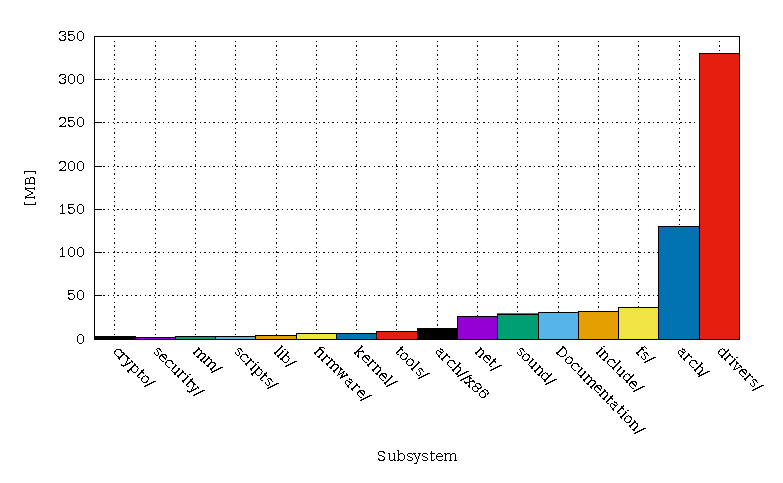
\includegraphics{plots/subsystemsizes.eps}
% \figb{Visualization of the sizes of the subsystems}{fig:subsystems}
% ---

The \texttt{drivers/} subsystem is by far the largest subsystem. It contains 
all hardware drivers. It is also mostly contributed to by hardware vendors.
    \footnote{Source? and is it true? -What would Greg Kroah Hartman say?}
Since it is the largest subsystem, one could suspect it to contain the most 
errors. And even when taking relative size into account, one could suspect this
on the grounds of the majority of the code being written by hardware vendors.
\\

The \texttt{arch/} subsystem contains architecture specific source code. 
There are 29 architectures in the \texttt{arch/} folder, which is why Linux is 
the operating system, which supports the most architectures in the world.
    \cite{22thbirthday}
.
\\

The \texttt{mm/} subsystem is for memory management, \texttt{security} is 
libraries regarding security, and \texttt{kernel} is the where the kernel 
specific code is. Other subsystems are \texttt{sound/}, \texttt{net/}, and 
\texttt{lib/}

% --- Not showing this graph ---
% \figa
%     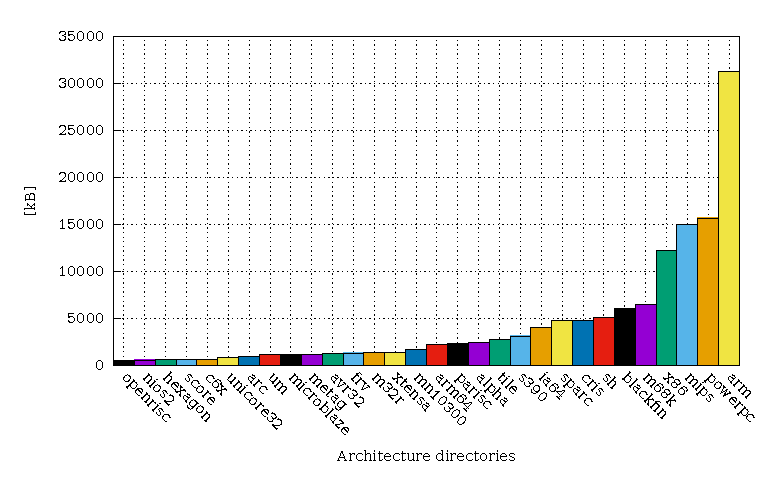
\includegraphics{plots/archsizes.eps}
% \figb{The sizes of the different architecture diretories}{fig:archsizes}
% ---


% TODO
\begin{itemize}
    \item \underline{\textbf{TODO}}
    \item Find out how to find the exact number of possible configurations. It 
        is in some article, I got by Andrzej. Plus maybe SharpSAT.
    \item Explain how to find the number of features by grepping.
    \item Talk about subsystems
    \item Maybe talk about the percentage of code in every subsystems. What is 
        Linux kernel made of?
    \item talk about who contributes to the kernel. (intel, novell). Both in 
        code and money?
    \item mention some more subsystems other than drivers and arch
\end{itemize}


        \subsection{Kconfig - The Language of the Feature Model}

            \paragraph{A feature model} 
is a way of representing all the possible configurations - \emph{the 
configuration space}. It contains all the features with their respective 
options and all the constraints and dependencies.

A feature model can be visualized in a feature diagram. The example given here 
will be tiny compared to that of the Linux kernel. The feature model of the 
Linux kernel is too big to fit in a normal sized report.

See figure \ref{featurediagramphone} for the toy example of a feature 
diagram. It 
depicts a feature model of a phone configuration, where there are some 
mandatory features and some optional, and also a choice option for the screen 
type. A cross-tree dependency is also present.

There is no consensus on a unified notation for attributes in feature models
    \cite{AAFM}
.

            \paragraph{The Kconfig language} 
is the language of the feature model in Linux (also used for other projects 
like BusyBox, BuildRoot, CoreBoot, Freetz and others)
    \cite[p. 4]{VarModSSD}
.
The configuration files have the prefix \textcode{Kconfig}, and are 
scattered all over the Linux kernel source code tree, where they include each 
other. There are 1195 Kconfig files in total in the Linux kernel
    \footnote{Found with the command \textcode{find . | grep Kconfig | wc}}
with 956 of them relevant for the \texttt{x86/} architecture.
\\

The different data types are \textcode{boolean}, \textcode{tristate}, 
\textcode{string}, \textcode{hex}, and \textcode{integer}. For a description of 
the context free grammar of the Kconfig language, see the appendices.
    \footnote{Write the Backus Naur Form of Kconfig in the Appendix}
\\



% 65 lines down to \figb
\figa
    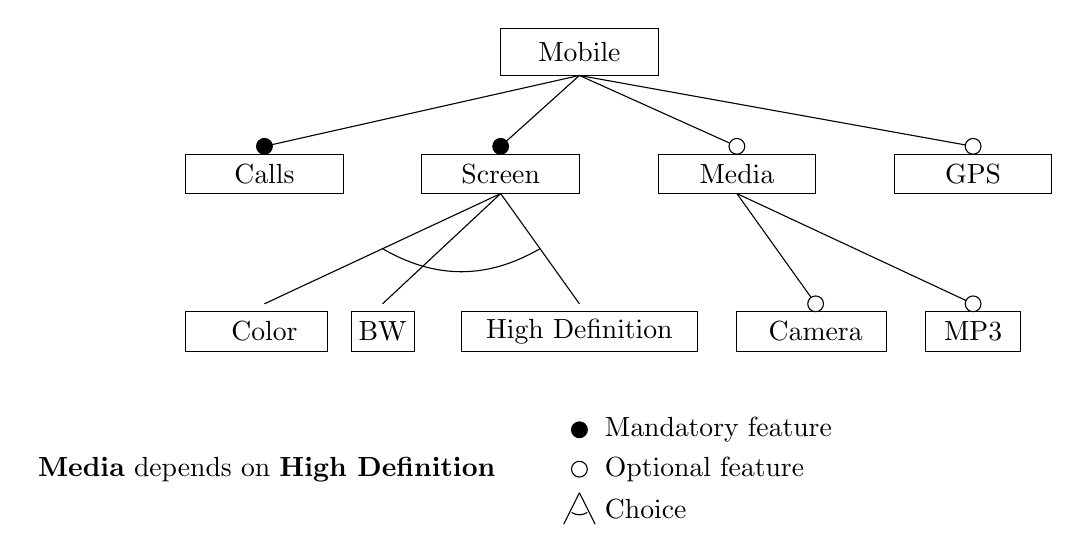
\begin{tikzpicture}
        % The top box
        \draw (3,3) rectangle (5,3.6);
        \draw (4,3.3) node {Mobile};

        % Middle words
        \draw (0.00,1.75) node {Calls};
        \draw (3,1.75) node {Screen};
        \draw (6,1.75) node {Media};
        \draw (9,1.75) node {GPS};

        % Middle edges
        \draw (0,2.1) edge (4,3);
        \draw (3,2.1) edge (4,3);
        \draw (6,2.1) edge (4,3);
        \draw (9,2.1) edge (4,3);

        % Middle dots
        \draw[fill=black] (0,2.1) circle (0.1);
        \draw[fill=black] (3,2.1) circle (0.1);
        \draw[fill=white] (6,2.1) circle (0.1);
        \draw[fill=white] (9,2.1) circle (0.1);

        % Middle boxes
        \draw (-1,1.5) rectangle (1,2);
        \draw (2,1.5) rectangle (4,2);
        \draw (5,1.5) rectangle (7,2);
        \draw (8,1.5) rectangle (10,2);

        % Bottom words
        \draw (0,-0.25) node {Color};
        \draw (1.5,-0.25) node {BW};
        \draw (4,-0.25) node {High Definition};
        \draw (7,-0.25) node {Camera};
        \draw (9,-0.25) node {MP3};

        % Bottom edges
        \draw (0,0.1) edge (3,1.5);
        \draw (1.5,0.1) edge (3,1.5);
        \draw (4,0.1) edge (3,1.5);
        \draw (7,0.1) edge (6,1.5);
        \draw (9,0.1) edge (6,1.5);

        % Bottom dots
        %\draw[fill=white] (0,0.1) circle (0.1);
        %\draw[fill=white] (2,0.1) circle (0.1);
        %\draw[fill=white] (4,0.1) circle (0.1);
        \draw[fill=white] (7,0.1) circle (0.1);
        \draw[fill=white] (9,0.1) circle (0.1);

        % The 'or'
        \draw (1.5,0.8) edge [bend right] (3.5,0.8);

        % Bottom boxes
        \draw (-1,-0.5) rectangle (0.8,0);
        \draw (1.1,-0.5) rectangle (1.9,0);
        \draw (2.5,-0.5) rectangle (5.5,0);
        \draw (6,-0.5) rectangle (7.9,0);
        \draw (8.4,-0.5) rectangle (9.6,0);


        % The legend
        \draw[fill=black] (4,-1.5) circle (0.1);
        \draw[fill=white] (4,-2) circle (0.1);
        \draw[right] (4.2,-1.5) node {Mandatory feature};
        \draw[right] (4.2,-2) node {Optional feature};

        \draw (4.0,-2.3) edge (4.2,-2.7);
        \draw (4.0,-2.3) edge (3.8,-2.7);
        \draw (4.1,-2.55) edge [bend left] (3.9,-2.55);
        \draw[right] (4.2,-2.5) node {Choice};

        % The cross-tree dependency
        \draw[right] (-3, -2) node {\textbf{Media} depends on 
            \textbf{High Definition}};

    \end{tikzpicture}
\figb{An example of a feature diagram of a phone}{featurediagramphone}
% 65 lines up to \figa


\figa
    \lstinputlisting[]{code/kconfigphone}
\figb{Kconfig for the phone example}{kconfigphone}

        {\color{gray}
The features in Kconfig can be split into four different types, \emph{User 
features}, \emph{Implementation features}, \emph{Derived features}, and 
\emph{Capability features}
    \cite[p. 8]{VarModSSD}
.
\\ 

\paragraph{User} features are features that the user chooses a value for in the 
configurator. In other words, a feature, that has a prompt option in the 
Kconfig language. 

These features may not directly inflict the compiler's choices, but may only 
open up for other features in the configurator.

\paragraph{Implementation} features are referenced in the source code, and will 
directly influence what code the preprocessor will select for compilation.

\paragraph{Derived} features are invisible to the user, and are set by other 
features using the \textcode{select FOO} syntax.

\paragraph{Capability} features in Linux are features, that simulate a reverse 
dependency. These features are also not randomly chosen by 
\texttt{randconfig}
    \footnote{Should I give an example here of the capability one?}
. Their names often start with \textcode{CONFIG\_HAVE\_} or 
\textcode{CONFIG\_ARCH\_HAVE\_}, and only have \emph{type} option set (often to 
\texttt{bool}).
        } % color gray

    \footnote{describe that all models are typically wide and shallow, VarModSSD page 19}
    \footnote{write how Kconfig is a beast sometimes. Child nodes exclusding their parents}
    \footnote{How many are there of each of these. distirbution.}



\begin{itemize}
    \item \underline{\textbf{TODO}}
    \item mention how many of boolean and tristate and so on, there are. Maybe 
            to use to say something about how many possible configurations can 
            be created.
    \item Explain the Kconfig language a bit
    \item Reference to Thorsten's projects
    \item Refer to the /Documentation/kbuild/kconfig-language.txt
    \item Should I have the Backus Naur Form of the Kconfig language here?
\end{itemize}

        \subsection{Configuring of Linux}

The Linux kernel comes with different ways of creating your own configuration 
file. There is a question based one (\texttt{config}), and some menu based ones 
(\texttt{menuconfig}, \texttt{xconfig}, \texttt{nconfig}, \texttt{gconfig}), 
but also some that will never prompt the user for anything, but create some 
automated config (\texttt{allyesconfig}, \texttt{allnoconfig}, 
\texttt{defconfig}, and \texttt{randconfig}).
\\

See figure \ref{fig:lineofconfigs} for a few examples of how the graphical 
configuration tools look.
\\


\figa
    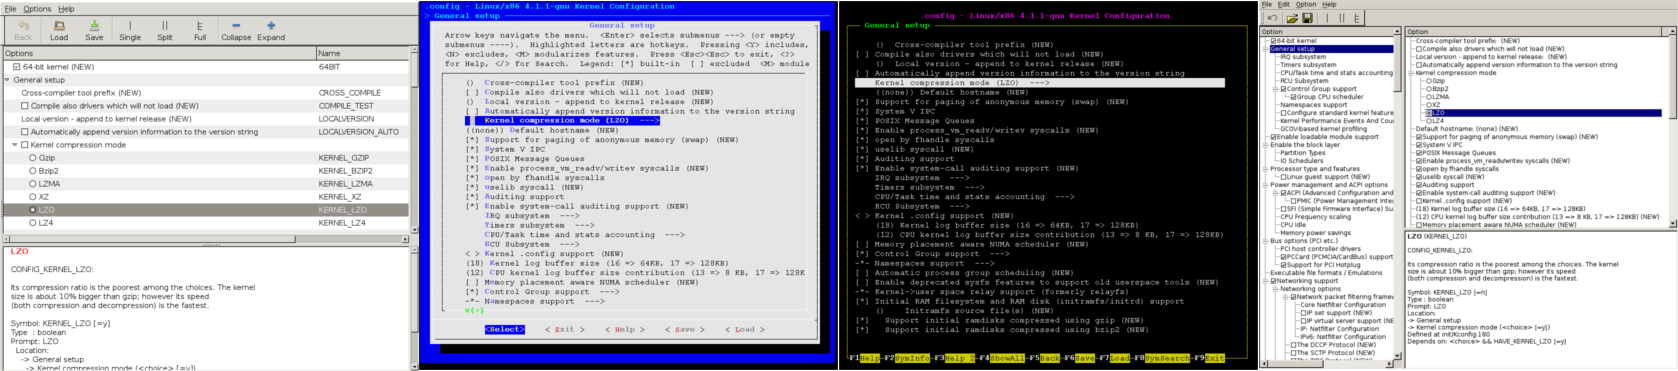
\includegraphics[scale=0.25]{pngs/configs50percent.png}
\figb{gconfig, menuconfig, nconfig, and xconfig}{fig:lineofconfigs}

\texttt{randconfig} is interesting, as it will go through the 
Kconfig feature model files, and pick random values for all of the features. 
This should be perfect for the goal for this project. Although time will tell 
that it is indeed biased, and will not create configurations that are of 
representative character. 

See figure ~\ref{randconfigtoy} for a toy example of a Kconfig feature model. 
It is a very small example with only two features, but it will easily explain 
some limitations of using \texttt{randconfig}.

\figa
    \lstinputlisting[language=C, firstline=1, morekeywords={prompt, config, 
        depends, on, bool, endchoice, choice,{||}}]{code/kconfigrandconfigtoy}
\figb{A toy Kconfig feature model}{randconfigtoy}

% --- 33 lines down ---
\figa
    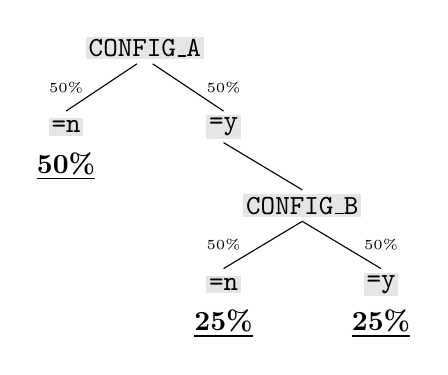
\begin{tikzpicture}
        % Names of configs
        \draw (2,4) node {\textcode{CONFIG\_A}};
        \draw (4,2) node {\textcode{CONFIG\_B}};

        % yeses and nos
        \draw (1,3) node {\textcode{=n}};
        \draw (3,3) node {\textcode{=y}};
        \draw (3,1) node {\textcode{=n}};
        \draw (5,1) node {\textcode{=y}};

        % lines not necessarily from above and down
        \draw[-] (1.9,3.8) edge (1,3.2);
        \draw[-] (2.1,3.8) edge (3,3.2);
        \draw[-] (3,2.8) edge (4,2.2);
        \draw[-] (3,1.2) edge (4,1.8);
        \draw[-] (5,1.2) edge (4,1.8);

        % Draw percentages
        \draw (1,3.5) node {\tiny{50\%}};
        \draw (3,3.5) node {\tiny{50\%}};
        \draw (3,1.5) node {\tiny{50\%}};
        \draw (5,1.5) node {\tiny{50\%}};

        \draw (1,2.5) node {\textbf{\underline{50\%}}};
        \draw (3,0.5) node {\textbf{\underline{25\%}}};
        \draw (5,0.5) node {\textbf{\underline{25\%}}};

    \end{tikzpicture}
\figb{A toy example showing the way randconfig selection of 
    features}{randconfigtoy50}
% --- 33 lines up ---

The example in figure ~\ref{randconfigtoy50} shows that the three possible 
configurations (\textcode{\{\}}, \textcode{\{A\}}, and \textcode{\{A,B\}}) do 
not have the same chance of getting created by \texttt{randconfig}.

For the creation to be representative, all the three possible configurations 
should have equal chance of being created (33\%). See figure 
~\ref{randconfigtoy33} for a visualization of how the selection should be to be 
representative.

% --- 32 lines up ---
\figa
    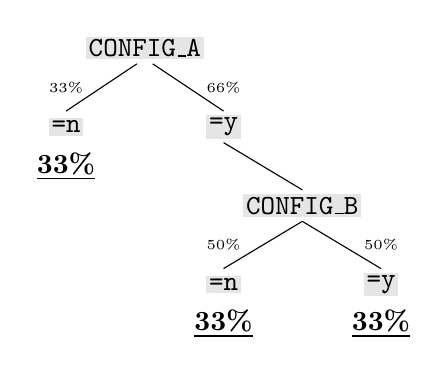
\begin{tikzpicture}
        % Names of configs
        \draw (2,4) node {\textcode{CONFIG\_A}};
        \draw (4,2) node {\textcode{CONFIG\_B}};

        % yeses and nos
        \draw (1,3) node {\textcode{=n}};
        \draw (3,3) node {\textcode{=y}};
        \draw (3,1) node {\textcode{=n}};
        \draw (5,1) node {\textcode{=y}};

        % lines not necessarily from above and down
        \draw[-] (1.9,3.8) edge (1,3.2);
        \draw[-] (2.1,3.8) edge (3,3.2);
        \draw[-] (3,2.8) edge (4,2.2);
        \draw[-] (3,1.2) edge (4,1.8);
        \draw[-] (5,1.2) edge (4,1.8);

        % Draw percentages
        \draw (1,3.5) node {\tiny{33\%}};
        \draw (3,3.5) node {\tiny{66\%}};
        \draw (3,1.5) node {\tiny{50\%}};
        \draw (5,1.5) node {\tiny{50\%}};

        \draw (1,2.5) node {\textbf{\underline{33\%}}};
        \draw (3,0.5) node {\textbf{\underline{33\%}}};
        \draw (5,0.5) node {\textbf{\underline{33\%}}};

    \end{tikzpicture}
\figb{A toy example showing a correct selection of features}{randconfigtoy33}
% --- 32 lines up ---

This has apparently not been implemented in the Linux kernel tools, possibly 
because representativeness does not matter for what it is used for. It is 
merely used as a simple fuzz testing tool with the help of entropy.
    \footnote{source}

To make this representative, one would have to make \texttt{randconfig} aware of
the whole dependency tree or the whole configuration space before randomly 
selecting, to skew the possibilities. This seems infeasible since the 
configuration space is so large. It will not fit in memory.
\\

Some different ways of generating a representative sample was considered. In 
the end, \texttt{randconfig} was chosen because it showed to be too cumbersome 
to create a method that actually was representative. 

The methods that was considered will be explained later in this report. 
See section \ref{sec:gen} on page \pageref{sec:gen}.
They included the aforementioned \texttt{randconfig} tool being rewritten, a 
script that \emph{scrambled the Kconfig} files, and a \emph{generate and 
filter} method.
\\



% TODO
\begin{itemize}
    \item \underline{\textbf{TODO}}
    \item .config file
    \item show results from running randconfig a 1000 times.
    \item Talk about how there is 7 layers of dependencies. And how I found out.
    \item \^ Hmm . Are there only 7 layers when counting ifs? what about 
        'depends on's
    \item mention that it is also called a preprocessor.
\end{itemize}


\subsection{Compiling and Catching Errors and Warnings}

When a configuration has been created, the Linux kernel is compiled using 
that configuration file by running the command \textcode{make all}
    \footnote{Or simply \textcode{make}, since \textcode{make all} is the 
        default behaviour}
. This looks in a \texttt{Makefile}, which specifies what files to compile. The 
compilation of the files is done mainly by \emph{gcc - The GNU Compiler 
Collection}
    footnote{Notice that both gcc version 4.9.2 and version 5.2.0 are used}
\\

During compilation, \texttt{gcc} will output warnings if there are any. These 
warnings warn about bad code, which might result in a compilation error, or 
which might result in dead code, or they might just warn about bad code 
practice.

These output messages hold the information that will be used in this project. 
In a warning, there is information about a possible coding mistake that might 
break the code. There are about 30 different warning types \cite{gccwarnings}
Some of these are not so interesting as others for this project.
\\

If there is an error, the compilation will stop immediately 
(at default it will try to keep on going, but in this project, it is told to 
stop after one error).
\\

Generally there will be distinguished between four different types of output. 
These are \textbf{Linux errors}, \textbf{host errors}, 
\textbf{relevant warnings}, and \textbf{irrelevant warnings}. 

The different types of output will be described here.


    \paragraph{The Linux errors} 
are reproducible errors that will occur on all 
machines when a certain configuration is being built. 
\\

In traditional bug finding, there are \emph{analysis-time}, 
\emph{compile-time}, and \emph{runtime}. With configurable software, there 
exists another one \emph{instantiation-time} or \emph{configuration-time}, 
which checks the preprocessing.
    \cite{IntDatSPL}

In this project \emph{compile-time} is in focus, and \emph{gcc} is both the 
compiler and in a sense, also the test-suite.
\\


    \footnote{Refer to the list of errors - some link somewhere}

    \paragraph{The host errors} 
are a result of the building system (a host system) not having some specific 
dependencies installed.
\\

For instance, there is a feature in the feature model that is called 
\textcode{CONFIG\_KERNEL\_LZO}, which dictates that the kernel should be 
compressed by the \emph{lzop} compression library instead of the default 
\emph{gzip} compression library.

If a configuration has the \textcode{CONFIG\_KERNEL\_LZO} enabled, then to 
build the kernel, the \emph{lzop} library will have to be installed on the 
build system. If it is not, then the compilation will stop with an error.

There are six different ways to compress the Linux kernel (\emph{gzip}, 
\emph{bzip2}, \emph{lzma}, \emph{xz}, \emph{lzo}, and \emph{lz4}),
which leads to that every sixth compilation will stop with the same error.

See figure \ref{fig:lineofconfigs} for an overview of how this specific choice
looks in the different graphical configurators..
\\

There exist many other examples like this in the Linux kernel where an 
uninstalled program will result in an unbuilt kernel. These \textbf{host 
errors} would have to be minimized, since they are not actual kernel errors, 
but local errors. 

On the build system for this project, the \emph{lzo} package was in the Linux 
distribution's repository, and therefore easy to install. The \emph{lz4} 
packager however was not.
\\

The following is a list of mandatory features, which are added to decrease the 
amount of host errors. In an early period of the project, it was found out that 
these specific features with specific values would stop the compilation every 
time.

It decreases the configuration space of this project, but otherwise 
would just give a lot of false positives.
\\

All these lines are added to the configurations, which are generated in
this project.

\begin{itemize}
    \item \textcode{CONFIG\_STANDALONE=y}
    \item \textcode{CONFIG\_FW\_LOADER=n}
    \item \textcode{CONFIG\_SECCOMP=y}
    \item \textcode{CONFIG\_PREVENT\_FIRMWARE\_BUILD=y}
    \item \textcode{CONFIG\_*LZ4*=n}
        \footnote{This means that all features having to do with \emph{lz4} 
                    were disabled}
\end{itemize}

See chapter~\ref{ch:ttv} about Threats to Validity on page \pageref{ch:ttv} 
for a more thorough description of the specific features.


    \paragraph{The relevant warnings}
are warnings that may cause an error at some point. The \emph{uninitialized 
variable} warning is such a warning. If a variable is uninitialized, and ends 
up being called, it may cause an error, and stop the compilation. See figure 
\ref{lst:uninitvar} for a code example.

The relevant warnings are:

\begin{itemize}
    \item Uninitialized variable
    \item Maybe uninitialized
    \item Overflow
    \item Deprecated declarations
        \footnote{Complete this list}
\end{itemize}

\figa
    \lstinputlisting[language=C, firstline=3]{code/uninitvar.c}
\figb{A toy program showing an uninitialized variable.}{lst:uninitvar}

If \textcode{CONFIG\_A} is not enabled in the program in figure 
~\ref{lst:uninitvar} it will return the warning 
'\texttt{'n' is used uninitialized in this function [-Wuninitialized]}' and the 
output, when the program is run, will be '\texttt{0Hello world}',
which is wrong, as the program was meant to output '\texttt{Hello World}'.

    \paragraph{The irrelevant warnings}
are warnings that will not stop the compilation, and will not make the program 
output wrong things. Warnings like \emph{unused function}, \emph{unused 
variable}, \emph{unused label}, and \emph{unused value}, will all end up as 
dead code, which is bad for fitting a kernel on some hardware with limited 
space. Apart from that it is nothing else than code pollution. See figure 
~\ref{lst:unusedvar} for a code example  of an unused variable.

The irrelevant warnings are:

\begin{itemize}
    \item Unused function
    \item Unused variable
    \item Unused label
    \item Unused value
        \footnote{Complete this list}
\end{itemize}

\figa
    \lstinputlisting[language=C, firstline=3]{code/unusedvar.c}
\figb{A program resulting in an unused variable warning.}{lst:unusedvar}

This will return the warning '\texttt{unused variable 'n' [-Wunused-variable]}'.

        \subsection{The Gcc Warnings}
Here follows a list of the warnings that was found during the compilations. 
They are ordered alphabetically.


            \paragraph{array-bounds}
is given, when gcc is certain that a subscript to an array is always out of 
bounds.

% See example in figure \ref{lst:arraybounds}.

% \figa
    % \lstinputlisting[language=C]{code/arraybounds}
% \figb{}{lst:arraybounds}


            \paragraph{cpp}
will show \textcode{\#warning} directives written in the code. This is a warning 
message that the coder can pass to the compiler. Often they will not result in 
an error.


            \paragraph{deprecated-declarations}
will show warnings when functions, variables, or types have been declared 
deprecated be a programmer.


            \paragraph{discarded-array-qualifiers}
            \paragraph{error=}
is a prefix, which means that the warning will cause an error. Sometimes 
developers do not want a specific warning to happen without the compilation 
stopping. Then they can enable this flag in the makefile.

There is also a \texttt{no-error=}, which nullifies the \texttt{error=} flag.


            \paragraph{frame-larger-than=}
            \paragraph{implicit-function-declaration}
            \paragraph{incompatible-pointer-types}
            \paragraph{int-conversion}
            \paragraph{int-to-pointer-cast}
\emph{See the section about pointer-to-int on page \pageref{par:pointertoint}}

            \paragraph{logical-not-parentheses}
occurs when the left hand side of an expression contains a \emph{logical not} 
(a \texttt{!} in C). An example is \textcode{if (!ret == template[i].fail)}
    \footnote{From the file \texttt{crypto/testmgr.c}}
.

The warning refers to the \textcode{!ret}, which should have been inside 
parentheses to be correct, like so \textcode{(!ret)}.


            \paragraph{maybe-uninitialized}
is when there is an uncertainty about a variable being uninitialized. In the 
case in figure \ref{lst:maybeuninitializedreal} there is a 
\texttt{switch-case} where \texttt{sgn} is not initialized in all of the cases.

If \emph{gcc} cannot see for sure that the variable is initialized, 
even if it would have been initialized in all of the cases, it will return this 
warning.

\figa
    \lstinputlisting[language=C]{code/maybeuninitializedreal}
\figb{A real example of maybe-uninitialized function}{lst:maybeuninitializedreal}


            \paragraph{overflow}


            \paragraph{pointer-to-int-cast}
            \label{par:pointertoint}
This warning would normally be sign of bad code. It is usually when a pointer 
is cast to a \texttt{long} and then later cast back into a function call. This 
is widely spread in Linux to simulate the effects of \emph{Object Oriented 
Programming}


            \paragraph{return-type}
            \paragraph{switch-bool}
            \paragraph{uninitialized}
            \paragraph{unused-function}
is a warning about a function that has never been called. This represents dead 
code, or code pollution. 

In the example in figure \ref{lst:unusedfuncreal}, the function 
\texttt{bq27x00\_powersupply\_unregister} will not be called if the feature 
\texttt{CONFIG\_BATTERY\_BQ27X00\_I2C} is not enabled, and is therefore an 
unused function.

\figa
    \lstinputlisting[language=C]{code/unusedfuncreal}
\figb{A real example of unused function - from the file 
    \texttt{drivers/power/bq27x00\_battery.c}}{lst:unusedfuncreal}


            \paragraph{unused-variable}
is basically the same as \texttt{unused-function}, but only with a variable 
instead of a function. There will be no example of this.


            \paragraph{unused-label}


% TODO
\begin{itemize}
    \item \underline{\textbf{TODO}}
\end{itemize}


%%%%%%%%%%%%%%%%%%%%%%%%%%%%%%%%%%%%%%%%%%%%%%%%%%%%%%%%%%%%%%%%%%%%%%%%%%%%%%%%
%                           METHODOLOGY
%%%%%%%%%%%%%%%%%%%%%%%%%%%%%%%%%%%%%%%%%%%%%%%%%%%%%%%%%%%%%%%%%%%%%%%%%%%%%%%%
\newpage
\chapter{Methodology}

The objective is to make a quantitative analysis of errors and warnings in the 
Linux kernel based on as many random configurations as are possible to generate 
within the time span of this project.

There will be generated random configurations, and these will be used to 
compile two different versions of the Linux kernel, a stable Linux kernel 
version \emph{4.1.1}, and a Linux kernel from the \emph{linux-next} repository.


\section{Research Questions}

\textbf{RQ1:} Will the unstable linux-next repository generate more errors than 
the stable kernel.

\textbf{RQ2:} In what subsystems do the most errors occur. And in the largest 
subsystems, in what subsubsystem? 
\\
It is likely that some errors or warnings are more severe than others, and some 
types of errors get fixed more than others. This leads to the next question.
\\


\textbf{RQ2:} What warnings are mostly generated.  
\\


And this can also be different between the stable and unstable versions. Hence 
the next question. 
\\


\textbf{RQ3:} What bugs seem to be fixed the most when going from unstable to 
stable. 
\\


As mentioned \footnote{Where is this mentioned about the subsystems? refer to 
it}, the subsystems of the kernel are of very different character. 
\footnote{mention somewhere earlier, that drivers are different from security 
or kernel} And therefore the bug types must differ from subsystem to subsystem. 
\\




\textbf{RQ5:} What percentage of the possible configurations for the Kernel are 
valid. 
\\


\textbf{RQ6:} Are there any specific features, that when enabled, will produce 
more warnings than others. 
\\




\section{Collecting data}

Every time a randomly configured compilation is running, \emph{gcc} will 
output warning and error messages in the \emph{standard error} output. This 
output is then scraped through to categorize it.

An output line will contain a \emph{bug type}, a \emph{filename}, \emph{line 
number}, and a \emph{message} describing the warning in english.


The collection of data has mainly been done on a computer at the IT University 
of Copenhagen. The computer has $32\times2.8 MHz$ and $128 GB$ of RAM, and the 
average time to compile a kernel and upload the data was around 1 minute and 35 
seconds. A fairly regular laptop with 4 cores and 8 GB of RAM does that in just 
over 8 minutes on average. 
\\


When a compilation is done, the output is scraped and categorized, and then 
uploaded to a database, for easy querying during and after the project. 

See the figures ~\ref{fig:conftable}, ~\ref{fig:bugstable}, and 
~\ref{fig:filestable} for the database tables.


\figa
    \begin{tabular}{c|c|c}
        \hline 
        \hline
        \multicolumn{3}{c}{\textbf{Configurations}} \\
        \hline
        \textbf{Name} & \textbf{Type} &\textbf{primary key} \\
        \hline
        hash & char(64) & primary key \\
        exit\_status & int(1) \\
        conf\_errs & text \\
        linux\_version & varchar(100) & primary key \\
        original & longtext \\
        \hline
        \hline
    \end{tabular}
\figb{The Configurations table}{fig:conftable}

\figa
    \begin{tabular}{c|c|c}
        \hline
        \hline
        \multicolumn{3}{c}{\textbf{Bugs}} \\
        \hline
        \textbf{Name} & \textbf{Type} &\textbf{primary key} \\
        \hline
        hash & char(64) & primary key \\
        type & varchar(50) \\
        linux\_version & varchar(100) \\
        config\_hash & char(64) \\
        subsystem & varchar(30) \\
        original & longtext \\
        \hline
        \hline
    \end{tabular}
\figb{The Bugs table referring to the Configurations table}{fig:bugstable}

\figa
    \begin{tabular}{c|c|c}
        \hline
        \hline
        \multicolumn{3}{c}{\textbf{Files}} \\
        \hline
        \textbf{Name} & \textbf{Type} &\textbf{primary key} \\
        \hline
        id & int(11) & primary key \\
        path & varchar(50) \\
        line & varchar(15) \\
        bug\_id & char(64) \\
        \hline
        \hline
    \end{tabular}
\figb{The Files table referring to the Bugs table}{fig:filestable}

% TODO
\begin{itemize}
    %\item Grepping the stderr
    \item Tell why we need to compile
    \item Tell about coccinelle, and why we dont use that
    \item Categorizing the warnings/Errors
    %\item About the collection machine
    %\item About the database setup
\end{itemize}




%%%%%%%%%%%%%%%%%%%%%%%%%%%%%%%%%%%%%%%%%%%%%%%%%%%%%%%%%%%%%%%%%%%%%%%%%%%%%%%%
%                               RESULTS
%%%%%%%%%%%%%%%%%%%%%%%%%%%%%%%%%%%%%%%%%%%%%%%%%%%%%%%%%%%%%%%%%%%%%%%%%%%%%%%%
\newpage
\chapter{Results}

A total of 42,060 configurations were compiled. Half of them from the unstable 
(linux-next) Linux version, and the other half a stable version of Linux 
(version 4.1.1).

    \section{Errors}

Out of 21,030 compilations, 7911 (38\%) of the unstable ones had an error and 
stopped. For the stable ones, it was 3611 (17\%), which had an error.

    \subsection{Stable}

Out of the 17\% of the compilations, that had errors, here is a sorted list of 
the warnings. To know exactly which warning is 'responsible' for the error, 
one would have to look into every case, and find out.
    \footnote{refer to GNU GCC warning options and also refer to the figure underneath}


\figa
    \begin{tabular}{c|c}
        \hline 
        \hline

        \textbf{Warning type} & \textbf{Percent} \\

        \hline

        unused-function & 57\% \\
        maybe-uninitialized & 45\% \\
        unused-variable & 35\% \\
        logical-not-parentheses & 34\% \\
        error=implicit-function-declaration & 27\% \\
        frame-larger-than= & 24\% \\
        cpp & 23\% \\
        pointer-to-int-cast & 20\% \\
        discarded-array-qualifiers & 19\% \\
        switch-bool & 17\% \\
        int-conversion & 14\% \\
        array-bounds & 14\% \\
        return-type & 12\% \\
        uninitialized & 12\% \\
        overflow & 11\% \\
        unused-label & 8.1\% \\
        deprecated-declarations & 5.4\% \\
        int-to-pointer-cast & 4.5\% \\
        implicit-function-declaration & 1.7\% \\
        incompatible-pointer-types & 0.44\% \\
        error=implicit-int & 0.17\% \\

        \hline 
        \hline
    \end{tabular}
\figb{The warnings distribution of the stable Linux of the compilations with 
    errors}{tab:stablewarnwitherrs}


    \subsection{Unstable vs.Stable}


    \section{Warnings}

In this section, it will be the warning distribution, not only for the ones 
with errors, which stopped compiling, but for all of the compilation.


    \subsection{Stable}

\figa
    \begin{tabular}{c|c}

    \end{tabular}
\figb{The warnings distribution of the stable Linux}{tab:stablewarn}


    \subsection{Unstable vs.Stable}


\section{Analyzing the data}


    \section{Number of valid configurations}

There was a hope, that something could be said about the percentage of valid 
configurations out of all possible combinations.

Some mandatory features were fixed, and an experiment was run, but after 100,000
configurations, none of them were valid. This can only be used to say something
about the upper bound of the percentage.


\section{Observations}


    \subsection{Configuration Warnings}
When creating a random configuration, 25\%
    \footnote{get the correct percentage}
of the times, it will output a warning about unmet dependencies. One might
suspect that configurations, which yielded a warning would result in
compilation errors. 

As can be seen in figure \ref{tbl:confwarns}, fewer of the stable kernels that 
had configuration warnings also had an error in the compilation. But the rise 
in erroneous compilations from configurations without config warnings to 
configurations with config warnings is very little, and is claimed irrelevant.

\figa
    \begin{tabular}{c|c|c}
    \hline
    \hline
        & \textbf{Stable} & \textbf{Unstable} \\
    \hline
    No config warnings & 17\% & 36\%\\
    Config warnings & 19\% & 40\%\\
    \hline
    \hline
    \end{tabular}
\figb{Percentage of the configs with and without warnings, which resulted in an 
    erroneous compilation}{tbl:confwarns}

% TODO
\begin{itemize}
    \item \underline{\textbf{TODO}}
\end{itemize}


%%%%%%%%%%%%%%%%%%%%%%%%%%%%%%%%%%%%%%%%%%%%%%%%%%%%%%%%%%%%%%%%%%%%%%%%%%%%%%%%
%                           THREATS TO VALIDITY
%%%%%%%%%%%%%%%%%%%%%%%%%%%%%%%%%%%%%%%%%%%%%%%%%%%%%%%%%%%%%%%%%%%%%%%%%%%%%%%%
\newpage
    \chapter{Threats to Validity}
\label{ch:ttv}

\emph{Blahblah about Threats to validity...}

\section{Generalization}
\label{sec:gen}

One major threat to validity is in the representativeness of the random 
configurations. Since the configurations are created using the \textcode{make 
randconfig} method, some configurations are more likely to be generated than 
others.

This means, that when something is generally said about all of the Linux 
Kernel, instead something is said about mostly a subset of Linuxes. See figure 
\ref{fig:repsubset} for a visualization of subsets which are both 
representative, and not representative.

\figa
    \emph{Show an image of true representativeness}
\figb{A representative subset}{fig:repsubset}

Three ways was thought of, that would make the configurations more 
generalizable. If successful with any of the methods, they could have been 
committed to the Linux kernel. Unfortunately, none of them were successful.


    \subsection*{Changing the code of \texttt{randconfig}}
The first idea was to change the code of \texttt{randconfig}, so it would know
what the possibilities of each outcome should be. See figure 
\ref{randconfigtoy33} for a visualization.

This was deemed impossible due to the very large feature model. The 
\emph{Abstract Syntax Tree (AST)} would simply not fit in memory of any 
computer.
    \footnote{Give short example}


    \subsection*{Permutation of Kconfig files}
Another idea was to take all the spread out Kconfig files, and concatenate 
them all into one big text file, which would then be modified and exposed to 
syntactic desugaring. If the order of the features were randomized, then the 
coins would not be flipped in the same order every time, and this could have an 
effect on the dependent features. 
\\

It turned out, that \texttt{randconfig} does not regard the order of the 
kconfig files. The Kconfig files are loaded, and \texttt{randconfig} then 
utilizes the AST and randomly selects from the root of that, which gives the
same result as when Kconfig is not permuted.


    \subsection*{Generate and Filter}
The third idea was to manually generate a configuration file, and then check - 
somehow - if the config file was valid, and then use it if it was valid. By 
not looking at dependencies, but only considering \emph{choice} options and 
enabling \emph{mandatory features}, a configuration file was created by 
randomly flipping a coin per each feature.

This seemed doable, but after generating 100,000 configurations, not one 
valid configuration was found.

It was considered running \emph{SharpSAT} (or \emph{\#SAT}) to count the number
of valid configurations, but it was deemed out of scope of this project.
    \footnote{Link to sharpSAT thingy}


    \subsection{Gcc versions}
Roughly a third of the compilations were done with gcc version 5.1.0 and two 
thirds with gcc version 4.9.2. This should not matter on what warnings are 
returned. There is only one new warning that is enabled by the \texttt{-Wall} 
flag in version 5.1.0
    \footnote{\texttt{-Wc++14compat}}
, and none of this type was found.


    \subsection{Architecture}

To create a true representative sample space, all the different architectures 
should be compiled for. There exist 31 different architectures, but the most 
common one for laptop and server use is the \texttt{x86} architecture.

This architecture is the only one, that are compiled for in this project, as 
getting the cross compilers for all the different architectures would be very 
cumbersome. 
\\


This potentially leaves out 97\% \footnote{is this number true. Should I 
calculate?} of the possible configurations to check.

\subsection{Firmware}

Some places in the kernel, there are drivers, which rely on some external 
proprietary binary blob, before they can be built. These binaries are not in 
the kernel, but would have to be downloaded specifically and put in certain 
folders in the kernel tree.

These are throwing errors, which are local errors, and therefore invalid. The 
task of getting all the drivers into the kernel tree was too great, so instead, 
those configurations are simply skipped.

This gives another bias in the sample, which now does not contain any 
configurations with these features on.


% --- 19 lines copied from further up
The feature \textcode{CONFIG\_STANDALONE} for instance, has been enabled in all 
the configurations in this project. If this feature is disabled, it allows for 
firmware drivers to be compiled in the kernel. But these firmware drivers are 
not open source, and must be placed in the kernel directories manually for the 
compilation to work.

Since it would be too cumbersome to find all the proprietary drivers, this 
option of enabling the \textcode{CONFIG\_STANDALONE} feature has been chosen, 
and will commit to a threat to validity in respect to representativeness.
\\

Also every feature that had some relation to the \emph{z4c} library has been 
diabled. This would require the host \footnote{explain what a host and target 
are at some point further up} to have this library installed. This library was 
not in the Linux distribution's repository, and it would have been too time 
consuming to have it installed. 

Therefore this also marks as a threat to validity.
% ---- 19 lines

\begin{itemize}
    %\item Only run on x86 architecture
    \item randconfig bias
    %\item firmware blobs
    \item Internal vs. External validity
    \item The mandatory features?
\end{itemize}

\section{Generate'n'Filter}



\begin{itemize}
    \item Uniform distribution
    \item Too low percentage
    \item Get a lower bound on the percentage
    \item sharpSAT?
\end{itemize}

\section{elvisconfig}


\section{RandomSAT}


% TODO
\begin{itemize}
    \item \underline{\textbf{TODO}}
    \item Maybe the permutation script can be used elsewhere (Thorsten seemed 
        interested)
\end{itemize}



%%%%%%%%%%%%%%%%%%%%%%%%%%%%%%%%%%%%%%%%%%%%%%%%%%%%%%%%%%%%%%%%%%%%%%%%%%%%%%%%
%                           RELATED WORK
%%%%%%%%%%%%%%%%%%%%%%%%%%%%%%%%%%%%%%%%%%%%%%%%%%%%%%%%%%%%%%%%%%%%%%%%%%%%%%%%
\newpage
\chapter{Related Work}

% TODO
\begin{itemize}
    \item \textbf{\underline{TODO}}
    \item 42 bugs
    \item Variability in ...
    \item Paper from Iago
    \item Fengguang Wu and Intel
\end{itemize}



\newpage
\chapter{Conclusion}
\emph{--- Leave empty until the end---}




\newpage
\bibliographystyle{plain}
\bibliography{bib}

\end{document}











% Example of Bibliography
\newpage
\bibliography{bibliography}

% Example of Appendix
\begin{appendices}
\chapter{Code}
\lstinputlisting[language=Python]{../temp.py}
\end{appendices}

% Example of a drawing
\begin{figure}[H]
    \begin{center}
        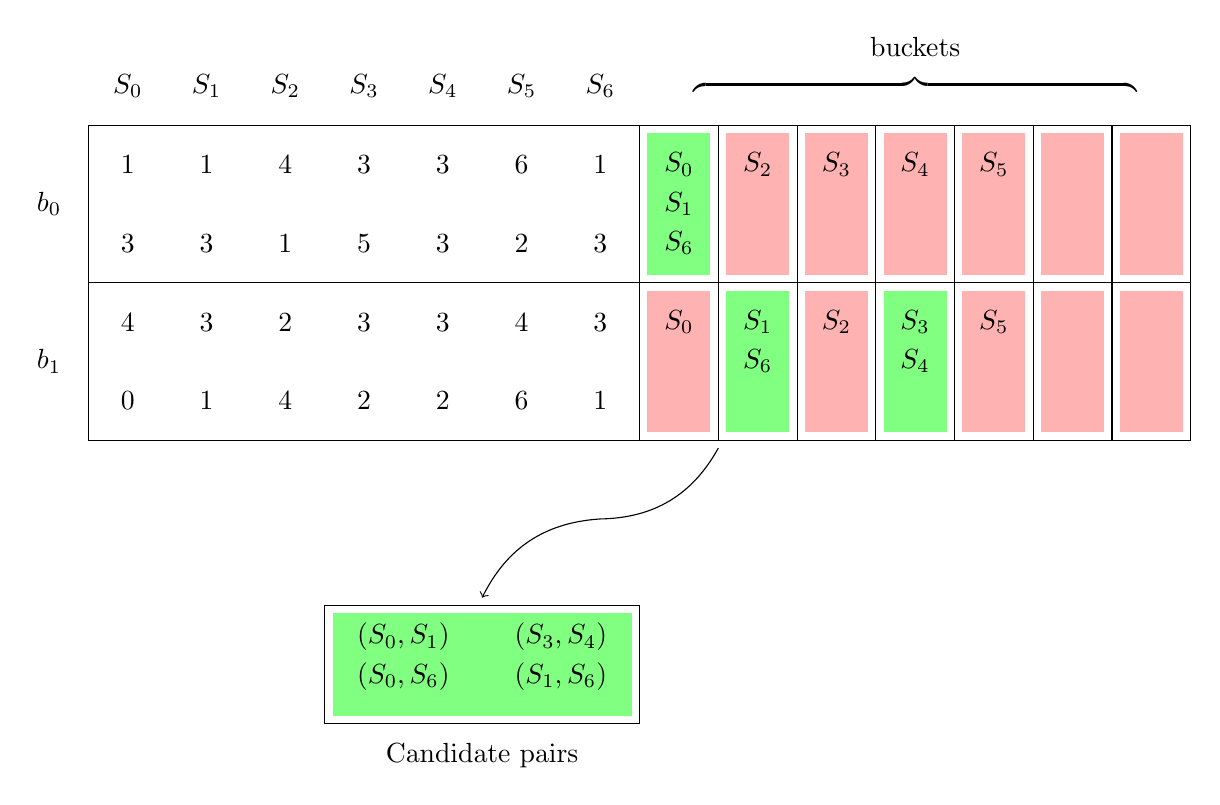
\begin{tikzpicture}
            \draw rectangle (14,4);
            \draw rectangle (7,2);
            \draw (0,2) rectangle (7,2);
            \draw (7,0) rectangle (8,4);

            \foreach \x in {0,...,6} \draw (\x+7, 0) rectangle (\x+7+1, 2);
            \foreach \x in {0,...,6} \draw (\x+7, 2) rectangle (\x+7+1, 4);
            \foreach \x in {0,...,6} \draw (\x+.5, 4.5) node {$S_\x$};

            \draw (-.5,3) node {$b_0$};
            \draw (-.5,1) node {$b_1$};

            % The overbrace
            \draw (10.5, 4.5) node {$\overbrace{\qquad\qquad\qquad\qquad\qquad\qquad\qquad\qquad}$};
            \draw (10.5,5.0) node {buckets};

            % Signature matrix (left part)
            \draw (0.5,3.5) node {1};
            \draw (0.5,2.5) node {3};
            \draw (0.5,1.5) node {4};
            \draw (0.5,0.5) node {0};

            \draw (1.5,3.5) node {1};
            \draw (1.5,2.5) node {3};
            \draw (1.5,1.5) node {3};
            \draw (1.5,0.5) node {1};

            \draw (2.5,3.5) node {4};
            \draw (2.5,2.5) node {1};
            \draw (2.5,1.5) node {2};
            \draw (2.5,0.5) node {4};

            \draw (3.5,3.5) node {3};
            \draw (3.5,2.5) node {5};
            \draw (3.5,1.5) node {3};
            \draw (3.5,0.5) node {2};

            \draw (4.5,3.5) node {3};
            \draw (4.5,2.5) node {3};
            \draw (4.5,1.5) node {3};
            \draw (4.5,0.5) node {2};

            \draw (5.5,3.5) node {6};
            \draw (5.5,2.5) node {2};
            \draw (5.5,1.5) node {4};
            \draw (5.5,0.5) node {6};

            \draw (6.5,3.5) node {1};
            \draw (6.5,2.5) node {3};
            \draw (6.5,1.5) node {3};
            \draw (6.5,0.5) node {1};

            % Fill all with red (in right part)
            \foreach \x in {0,...,6} \path[fill=red!30] (7.1+\x,0.1) rectangle (7.9+\x,1.9);
            \foreach \x in {0,...,6} \path[fill=red!30] (7.1+\x,2.1) rectangle (7.9+\x,3.9);

            % Fill the right ones with green
            \path[fill=green!50] (7.1,2.1) rectangle (7.9,3.9);
            \path[fill=green!50] (8.1,0.1) rectangle (8.9,1.9);
            \path[fill=green!50] (10.1,0.1) rectangle (10.9,1.9);

            % Names
            \draw (7.5,3.5) node {$S_0$};
            \draw (7.5,3.0) node {$S_1$};
            \draw (7.5,2.5) node {$S_6$};
            \draw (8.5,3.5) node {$S_2$};
            \draw (9.5,3.5) node {$S_3$};
            \draw (10.5,3.5) node {$S_4$};
            \draw (11.5,3.5) node {$S_5$};

            \draw (7.5,1.5) node {$S_0$};
            \draw (8.5,1.5) node {$S_1$};
            \draw (8.5,1.0) node {$S_6$};
            \draw (9.5,1.5) node {$S_2$};
            \draw (10.5,1.5) node {$S_3$};
            \draw (10.5,1.0) node {$S_4$};
            \draw (11.5,1.5) node {$S_5$};


            % Arrows
            \path[-] (8,-.1) edge [bend left] (6.5,-1);
            \path[->] (6.5,-1) edge [bend right] (5,-2);

            % Candidate squares
            \path[fill=green!50] (3.1, -3.5) rectangle (6.9, -2.2);
            \draw (3,-3.6) rectangle (7,-2.1);

            % Candidate signatures
            \draw (4,-2.5) node {$(S_0, S_1)$};
            \draw (4,-3.0) node {$(S_0, S_6)$};
            \draw (6,-3.0) node {$(S_1, S_6)$};
            \draw (6,-2.5) node {$(S_3, S_4)$};

            \draw (5,-4.0) node {Candidate pairs};
            

        \end{tikzpicture}
    \caption{LSH buckets and bands}
    \label{fig:lsh_buckets}
    \end{center}
\end{figure}


% Example of algorithm
\begin{center}   
    \captionof{algorithm}{Locality Sensitive Hashing algorithm}\label{alg:lsh}
    \begin{algorithmic}
    
    \BState \textbf{Calculate signature matrix as in algorithm \ref{alg:minhashing}}\\

    \State $SIG\gets \text{signature matrix}$
    \State $S\gets \text{number of signatures}$
    \State $bucket\_list\gets \text{empty list}$
    \State $B\gets \text{number of bands}$\\

    \BState \emph{Fill the buckets}
    \For{$b_i$ in $i = 0 \ldots B-1$}
        \State $h_i \gets \text{empty dictionary}$
        \State $bucket\_list.append(h_i)$
        \For{$SIG_j[b_i]$ in $j = 0 \ldots S-1$}
            \State $key \gets SIG_j[b_i]$
            \If{$key$ in $h_i$}
                \State $bucket \gets h_i[key]$
            \Else
                \State $bucket \gets \text{empty list}$
            \EndIf
            \State $bucket.append(j)$
        \EndFor
    \EndFor\\

    \State $candidate\_pairs \gets \text{empty set}$
    \ForAll{$h_i$ in $bucket\_list$}
        \ForAll{$key$ in $h_i$}
            \State $bucket \gets h_i[key]$
            \If{$bucket.length > 1$}
                \For{$pair$ in $bucket$}
                    \State $candidate\_pairs.add(pair)$ 
                \EndFor
            \EndIf
        \EndFor        
    \EndFor\\

    \BState \textbf{Calculate similarities from signature matrix as in algorithm \ref{alg:minhashing}, for the candidate pairs.}

    \end{algorithmic}
\end{center}


% Example of a gnuplot input
\begin{figure}[H]
    \begin{center}
        \input{plots/scurve.tex}
        \caption{S-curve - $f(s) = 1 - (1 - s^r)^b$ ; $k = 1000$}
        \label{fig:scurve}
    \end{center}
\end{figure}


% Example of a table
\begin{figure}[H]
    \begin{center}
        \begin{tabular}{c|c|c}
              & Actual & LSH \\
            \hline
            1 & 1.0 & 1.0 \\
            2 & 1.0  & 1.0 \\
            3 & 0.667 & 0.702 \\
            4 & 0.667 & 0.695 \\
            5 & 0.667 & 0.689 \\
            6 & 0.667 & 0.684 \\
            7 & 0.667 & 0.681 \\
            8 & 0.667 & 0.681 \\
            9 & 0.667 & 0.677 \\
            10 & 0.667 & 0.673 
        \end{tabular}
        \caption{Correctness of LSH}
        \label{tab:lsh-correctness}
    \end{center}
\end{figure}


% Example of equation
\begin{equation}
    \frac{B(64;R,r_1,r_2)}{B(1;R,r_1,r_2} \Rightarrow \frac{64 R}{R + 1 - r_1}
    \label{eq:improvementratio}
\end{equation}


% Example of graphic
\begin{figure}[H]
    \begin{center}
        \includegraphics{plots/bbit/bbit.eps}
        \caption{b-Bit storage improvement}
        \label{fig:bbit}
    \end{center}
\end{figure}
